\documentclass[
	% -- opções da classe memoir --
	12pt,				% tamanho da fonte
	openright,			% capítulos começam em pág ímpar (insere página vazia caso preciso)
% 	twoside,			% para impressão em verso e anverso. Oposto a oneside
% 	openany,
	oneside,
	a4paper,			% tamanho do papel. 
	% -- opções da classe abntex2 --
	chapter=TITLE,			% títulos de capítulos convertidos em letras maiúsculas
	%section=TITLE,			% títulos de seções convertidos em letras maiúsculas
	%subsection=TITLE,		% títulos de subseções convertidos em letras maiúsculas
	%subsubsection=TITLE,% títulos de subsubseções convertidos em letras maiúsculas
	% -- opções do pacote babel --
	english,			% idioma adicional para hifenização
	french,				% idioma adicional para hifenização
	spanish,			% idioma adicional para hifenização
	brazil				% o último idioma é o principal do documento
	]{abntex2}

% ---
% PACOTES
% ---
%usa o arquivo unijui.sty com as alterações
\usepackage{unijui}
\usepackage{titlesec}
\usepackage{graphicx}
\titleformat{\section}{\normalfont\fontsize{12}{19}\Large\bfseries}{\thesection}{1em}{}
\titleformat{\subsection}{\normalfont\fontsize{12}{19}\large\bfseries\slshape}{\thesubsection}{1em}{}
\titleformat{\subsubsection}{\normalfont\fontsize{12}{19}\normalsize\slshape}{\thesubsubsection}{1em}{}

% ---
% Pacotes fundamentais 
% ---
\usepackage{lmodern}			% Usa a fonte Latin Modern			
\usepackage[T1]{fontenc}		% Selecao de codigos de fonte.
\usepackage[utf8]{inputenc}		% Codificacao do documento (conversão automática dos acentos)
\usepackage{lastpage}			% Usado pela Ficha catalográfica
\usepackage{indentfirst}		% Indenta o primeiro parágrafo de cada seção.
\usepackage{color}				% Controle das cores
\usepackage{graphicx}			% Inclusão de gráficos
\usepackage{microtype} 			% para melhorias de justificação
\usepackage{subcaption}			% sub-legenda
\usepackage{tabularx}			% tabelas melhores
\usepackage{float} 				% posicionamento de elementos
% ---
\renewcommand{\rmdefault}{phv} % Arial
\renewcommand{\sfdefault}{phv} % Arial
%\usepackage[scaled]{helvet}		%Usa a fonte helvética
\renewcommand*\familydefault{\sfdefault} %% Only if the base font of the document is to be sans serif
\usepackage[T1]{fontenc}

% ---
% Pacote Listings
% ---
\usepackage{listings}
\lstset{frame=tb,
  aboveskip=3mm,
  belowskip=3mm,
  showstringspaces=false,
  columns=flexible,
  basicstyle={\small\ttfamily},
  numbers=none,
  numberstyle=\tiny\color{gray},
  keywordstyle=\color{blue},
  commentstyle=\color{dkgreen},
  stringstyle=\color{mauve},
  breaklines=true,
  breakatwhitespace=true,
  tabsize=3
}

% --- Cores personalizadas
\definecolor{dkgreen}{rgb}{0,0.6,0}
\definecolor{gray}{rgb}{0.5,0.5,0.5}
\definecolor{mauve}{rgb}{0.58,0,0.82}
		
% ---
% Pacotes adicionais, usados apenas no âmbito do Modelo Canônico do abnteX2
% ---
\usepackage{lipsum}				% para geração de dummy text
% ---
% ---
% Pacotes de citações
% ---
\usepackage[brazilian,hyperpageref]{backref}	 % Paginas com as citações na bibl
\usepackage[alf]{abntex2cite}	% Citações padrão ABNT
%\usepackage{caption}

% --- 
% CONFIGURAÇÕES DE PACOTES
% --- 


% ---
% Configurações do pacote backref
% Usado sem a opção hyperpageref de backref
\renewcommand{\backrefpagesname}{Citado na(s) página(s):~}
% Texto padrão antes do número das páginas
\renewcommand{\backref}{}
% Define os textos da citação
\renewcommand*{\backrefalt}[4]{
	\ifcase #1 %
		%Nenhuma citação no texto.%
	\or
		%Citado na página #2.%
	\else
		%Citado #1 vezes nas páginas #2.%
	\fi}%
% ---

% ---
% Informações de dados para CAPA e FOLHA DE ROSTO
% ---
\titulo{Implementação de Sistema de Ponto com Arduino e Android}
\autor{MATHIAS HENRIQUE NAST BERWIG}
\local{Ijuí}
\data{2016}

\instituicao{%
 UNIVERSIDADE REGIONAL DO NOROESTE DO ESTADO DO RIO GRANDE DO SUL\par
   DEPARTAMENTO DE CIÊNCIAS EXATAS E ENGENHARIAS\par
   CIÊNCIA DA COMPUTAÇÃO
  }
\tipotrabalho{Trabalho Acadêmico}

% Configurações de aparência do PDF final

% alterando o aspecto da cor azul
\definecolor{blue}{RGB}{41,5,195}

% informações do PDF
\makeatletter
\hypersetup{
     	%pagebackref=true,
		pdftitle={\@title}, 
		pdfauthor={\@author},
    	pdfsubject={\imprimirpreambulo},
	    pdfcreator={LaTeX with abnTeX2},
		pdfkeywords={abnt}{latex}{abntex}{abntex2}{trabalho acadêmico}, 
		colorlinks=true,       		% false: boxed links; true: colored links
    	linkcolor=black,          	% color of internal links
    	citecolor=black,        		% color of links to bibliography
    	filecolor=magenta,      		% color of file links
		urlcolor=blue,
		bookmarksdepth=4
}
\makeatother
% --- 

% --- 
% Espaçamentos entre linhas e parágrafos 
% --- 

% O tamanho do parágrafo é dado por:
\setlength{\parindent}{1.5cm}

% Controle do espaçamento entre um parágrafo e outro:
\setlength{\parskip}{0.25cm}  % tente também \onelineskip

% ---
% compila o indice
% ---
\makeindex
% ---

%\usepackage{fancyhdr}
%\fancyhead{}
%\fancyfoot{}
%\lhead{}
%\rhead{\thepage}

%
%\fancypagestyle{ultima}{
%	\fancyhead{}
%	\fancyfoot{}
%	\lhead{}
%	\rhead{\thepage}
%	\rfoot{}
%}

% ----
% Início do documento
% ----
\begin{document}

% Retira espaço extra obsoleto entre as frases.
\frenchspacing 

% ----------------------------------------------------------
% ELEMENTOS PRÉ-TEXTUAIS
% ----------------------------------------------------------
 \pretextual

% ---
% Capa
% ---

\imprimircapa

% inserir o sumario
% ---
\pdfbookmark[0]{\contentsname}{toc}
\tableofcontents*
\cleardoublepage
% ---

% ----------------------------------------------------------
% TEXTO
% ----------------------------------------------------------

\pagestyle{simple} %PARA INICIAR CONTAGEM DE LPAGINAS
\chapter{Introdução}
\label{introducao}

Durante a disciplina de Programação de Sistemas Básicos, ministrada pelo Professor Marcos Cavalheiro na Universidade Regional do Noroeste do Estado do Rio Grande do Sul, foi solicitada como atividade avaliativa a implementação de um sistema de controle de ponto eletrônico utilizando a dispositivos Arduino. 

O objetivo do trabalho desenvolvido é construir e implementar um sistema capaz de, por meio de cartões identificados por radiofrequência (RFID), controlar a entrada e saída de estudantes de uma universidade. Com a proposta de qualificar o serviço, o autor deste trabalho optou por utilizar também um aplicativo Android para realizar o acompanhamento dos registros.
\chapter{Metodologia}
\label{metodologia}

A metodologia de desenvolvimento foi escolhida em razão das necessidades específicas da universidade. Ao longo deste capítulo será possível entender a situação problema apresentada, os recursos disponíveis para a resolução do mesmo e a implementação do sistema de controle de ponto.

\section{Problema}

Uma certa universidade oferece bolsas de pesquisa e extensão para seus alunos. Para realizar o controle de presença dos mesmos, é utilizado um sistema manual de registro ponto, onde é necessário que o estudante visite a secretaria da instituição e assine um documento de modo a comprovar sua presença.

Buscando otimizar esse processo, a universidade busca implantar um sistema mais prático de controle de ponto. Deste modo, foi realizada análise da rotina diária destes bolsistas e constatado que cada um possui horários de entrada e saída diferenciados. Com base nessas informações, o autor deve construir e implementar um sistema eletrônico de controle de ponto.
\section{Recursos Disponíveis}

A instituição dispõe dos seguintes recursos para a implantação do sistema:
\begin{itemize}
\item 1 Kit módulo leitor RFID, composto por duas TAGs (cartão e chaveiro);
\item 1 Arduino Uno;
\item 1 Arduino Mega;
\item 1 Ethernet Shield para Arduino;
\item 1 Protoboard.
\end{itemize}
\section{Modo de Implementação}

Para atender os requisitos solicitados pela universidade, o sistema será desenvolvido em 3 módulos, sendo eles: unidade Arduino, servidor e aplicativo Android. Estes módulos podem funcionar de modo interligado, exigindo conexão permanente entre os dispositivos.

O módulo Arduino será composto pelos Arduinos Uno e Mega, que serão responsáveis por interligar o sensor RFID e os LEDs indicadores. Quando o usuário passar seu cartão junto ao leitor, o Arduino Uno deve ler a TAG do cartão, envia-la para o Arduino Mega e este fazer o registro junto ao servidor. Para indicar se o ponto foi registrado corretamente o LED verde ficará aceso por 1 segundo, do contrário, o vermelho ligará pelo mesmo período de tempo.

O módulo servidor será responsável por gerenciar as informações relacionadas ao controle de ponto e usuário. Ele ficará instalado em um computador conectado à internet com um serviço de banco de dados e outro de web. Estes atenderão as requisições do Arduino Mega e do Android.

O aplicativo Android será capaz de exibir as informações consultadas no servidor. Para isso, ele deve possuir uma tela com a listagem de registros de ponto, com opções para filtrar por pessoa ou período (data de início e data de fim).
\chapter{Implementação}
\label{implementacao}

Este capítulo detalha os aspectos da implementação do sistema de controle de ponto. Nele estão expostas as particularidades do banco de dados, servidor web, arduino e aplicativo Android.

\section{Banco de Dados}

Como requisito funcional é necessário armazenar as informações de modo não volátil, optou-se por utilizar um banco de dados relacional. Devido a praticidade encontrada e conhecimento prévio do autor, a tecnologia utilizada para tal foi a do \textit{MySQL}.

Para a realização de um registro de ponto eletrônico, duas entidades estão envolvidas: a pessoa responsável por registrar o ponto, e o próprio ponto. A relação é de 1-n, ou seja: uma pessoa pode ter múltiplos pontos, mas um ponto pode pertencer a apenas uma pessoa.

Cada pessoa possui um nome e uma foto, e é identificada unicamente por sua tag (o número de série de seu cartão ponto). Cada registro de ponto possui um identificador único de chave primária, uma tag referenciando uma pessoa, e a data e hora que o ponto foi registrado. A figura ~\ref{diagrama_er} demonstra as relações citadas.

\begin{figure}[h]
	\centering
	\caption{Diagrama de Entidade-Relacionamento do Banco de Dados.}
	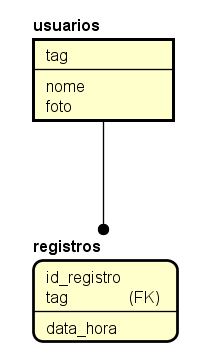
\includegraphics[scale=1]{imagens/bd_diagrama_er.png}
	\label{diagrama_er}
\end{figure}

Os tipos de dados foram escolhidos de modo a simplificar sua implementação em outras plataformas. Veja abaixo o \textit{script} de criação do banco de dados.

\renewcommand{\lstlistingname}{Código}
\begin{lstlisting}[language=SQL, label=bd_criacao, caption=Código de criação do banco de dados.]
DROP DATABASE IF EXISTS ponto;
CREATE DATABASE ponto;
USE ponto;

-- TABELA usuarios
DROP TABLE IF EXISTS usuarios;
CREATE TABLE usuarios (
 tag VARCHAR(10) NOT NULL,
 nome VARCHAR(64) NOT NULL,
 foto VARCHAR(256) NOT NULL,
 PRIMARY KEY (tag)
);

-- TABELA registros
DROP TABLE IF EXISTS registros;
CREATE TABLE registros (
 id_registro INT NOT NULL AUTO_INCREMENT,
 tag VARCHAR(10) NOT NULL,
 data_hora TIMESTAMP,
 PRIMARY KEY (id_registro),
 FOREIGN KEY (tag) REFERENCES usuarios (tag)
);
\end{lstlisting}
\section{Servidor Web}

O servidor web é responsável por atender as solicitações de registro de ponto do Arduino e consulta do Android. Para isso, a tecnologia empregada no desenvolvimento do web server foi o Apache, uma plataforma de servidor gratuita e de código aberta. 

Para atender os requisitos mínimos da aplicação forma necessários apenas três métodos com algumas variações, totalizando cinco rotinas diferentes. A tabela ~\ref{ws_tabela_metodos} demonstra esses métodos e os respectivos retornos.

\begin{table}[H]
\caption{Métodos suportados pelo servidor web.}
\label{ws_tabela_metodos}
\begin{tabularx}{\textwidth}{|c|c|c|X|}
\hline
\textbf{Nome do Método} & \textbf{Requisição Suportada} & \textbf{Parâmetros} & \multicolumn{1}{c|}{\textbf{Retorno}} \\ \hline
registrarPonto & POST & tag & HTTP Code: 201 (sucesso) ou 400 (falha). \\ \hline
getUsuarios & GET & - & Todos os usuários cadastrados. \\ \hline
getRegistros & GET & - & Todos os registros de ponto. \\ \hline
getRegistros & GET & tag & Todos os registros de ponto para a tag informada. \\ \hline
getRegistros & GET & dataInicio, dataFim & Todos os registros de ponto entre a data e hora informados. \\ \hline
\end{tabularx}
\end{table}

Os métodos do tipo \textit{GET} realizam uma consulta no banco de dados, filtrando os resultados de acordo com os parâmetros informados e então retornam as informações em formato \textit{JSON}. O método \textit{registrarPonto} é responsável por realizar uma operação de inserção no banco de dados, e seu retorno é em formato de código HTTP. Caso a inserção tenha sido realizada com sucesso, o mesmo retorna o código 201. Do contrário, 400.
\section{Arduino}

O Arduino Uno e o Arduino Mega são responsáveis pela leitura do registro de ponto. Os dois são interligados por meio das portas seriais. O Arduino Uno é ligado diretamente ao sensor RFID e recebe os bytes informando o valor da tag sempre que uma leitura é realizada. Em seguida, ele transfere esses dados para o Arduino Mega, que envia uma requisição POST ao servidor web, solicitando que o registro de ponto seja criado. De acordo com a resposta do servidor (que pode ser um código HTTP 201 no caso de sucesso, ou 400 para falha), um LED é ligado na protoboard (verde para sucesso ou vermelho para falha). Assim, ao passar cartão, o estudante tem uma resposta visual praticamente imediata. 

Na figura ~\ref{arduino_esquema} é possível notar a simplicidade do projeto: ele conta com apenas alguns pequenos componentes e é bastante flexível. 

\begin{figure}[H]
	\centering
	\caption{Esquema de ligação dos componentes eletrônicos.}
	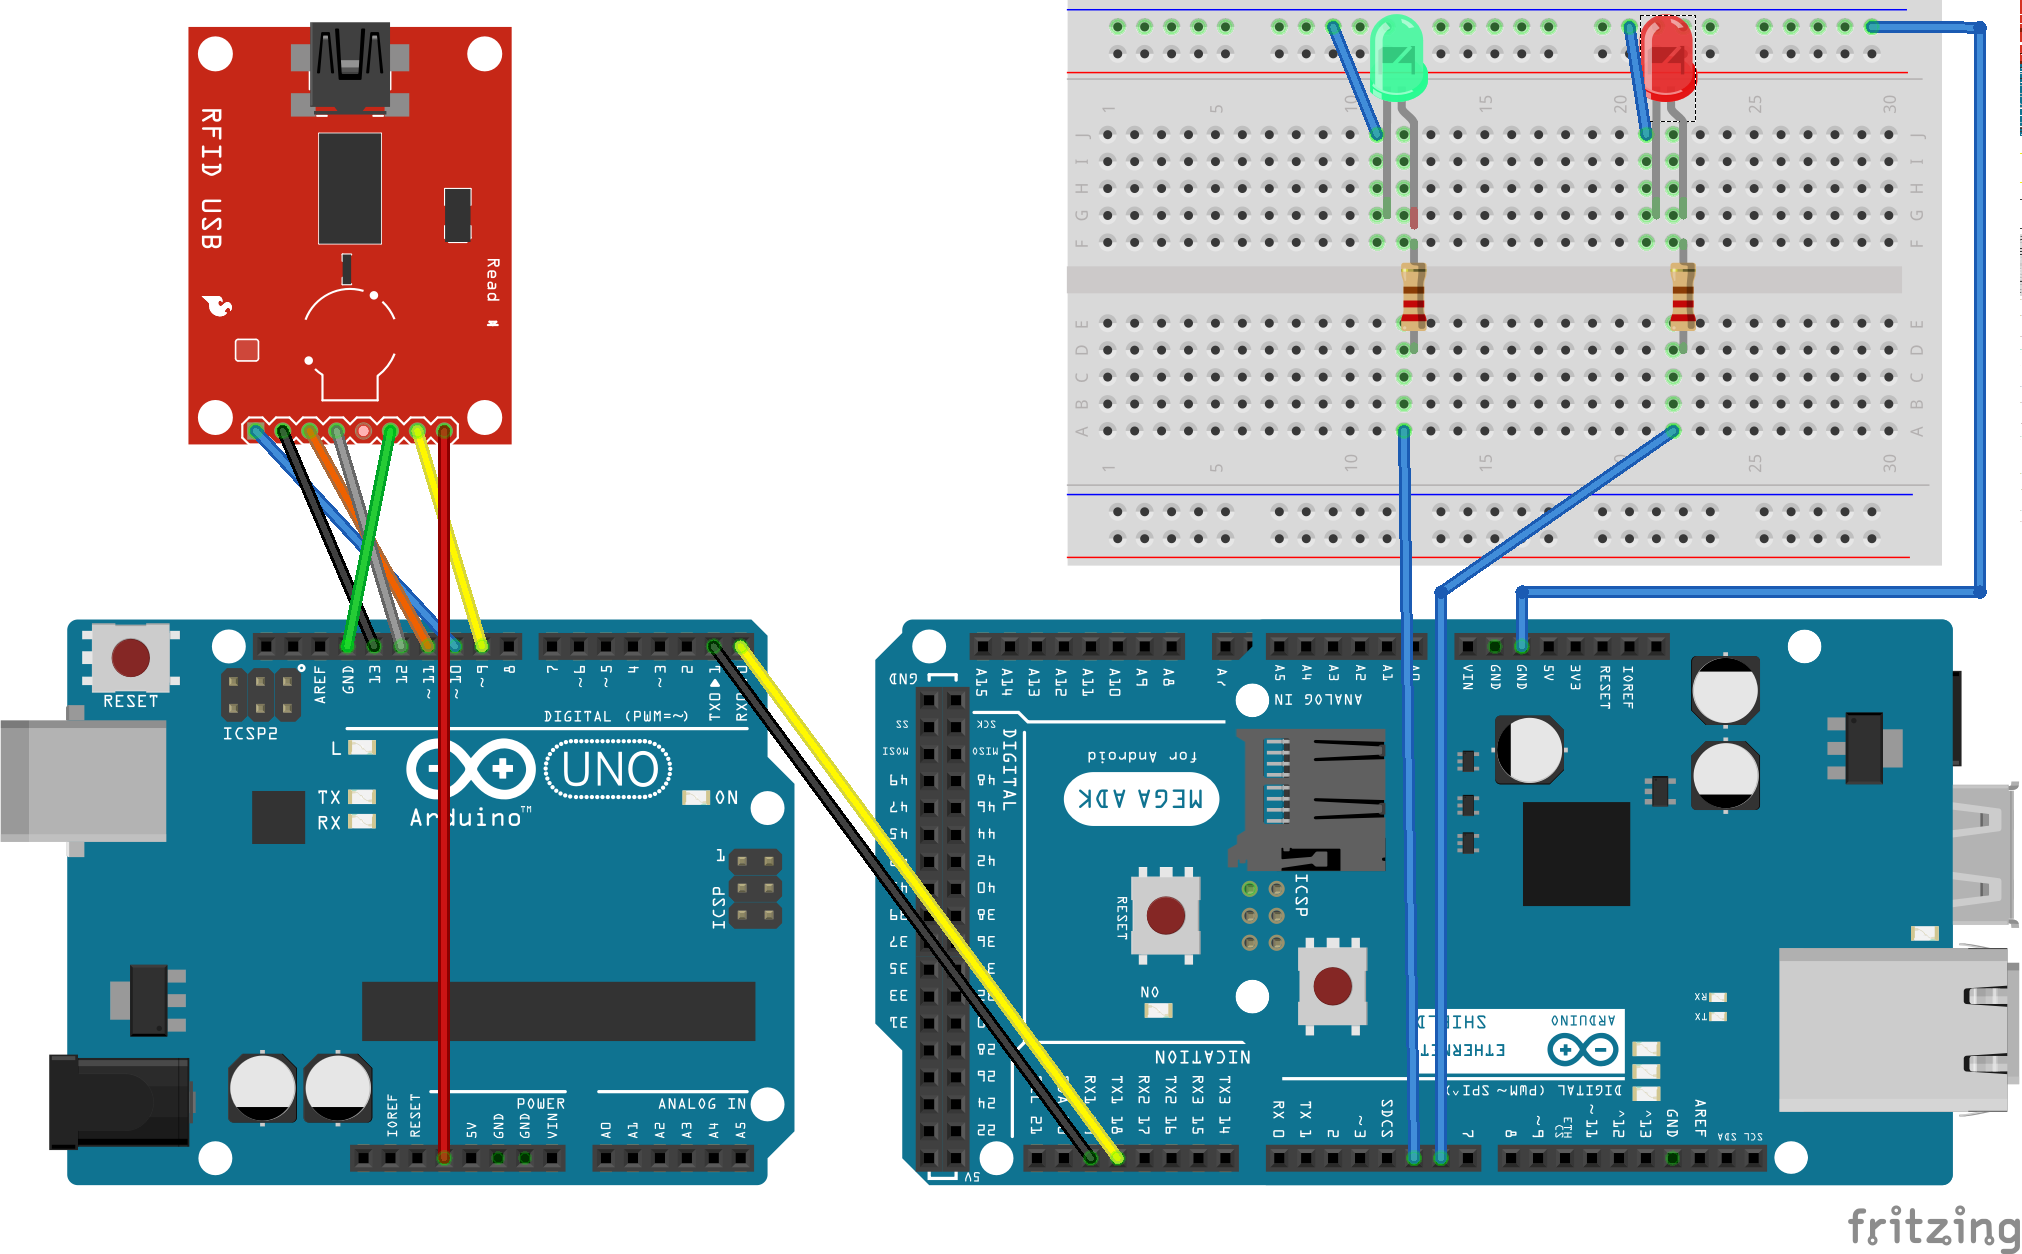
\includegraphics[scale=0.8]{imagens/arduino_esquema.png}
	\label{arduino_esquema}
\end{figure}
\section{Android}

O aplicativo Android é responsável por exibir as informações do servidor web de forma prática e rápida. Ele é compatível versões do sistema superiores ao 4.1 (SDK 16) e possui apenas uma tela. 

Por meio de consultas ao servidor web, o aplicativo lista os registros de ponto. Ele  filtrar os resultados por pessoa, por período (com data de início e data de fim) e também atualizar as informações da consulta que está sendo exibida.

A ~\ref{android_screenshots} mostra as opções disponíveis no aplicativo.

\begin{figure}
\centering
\begin{subfigure}{.5\textwidth}
	\centering
	\caption{Tela Inicial}
	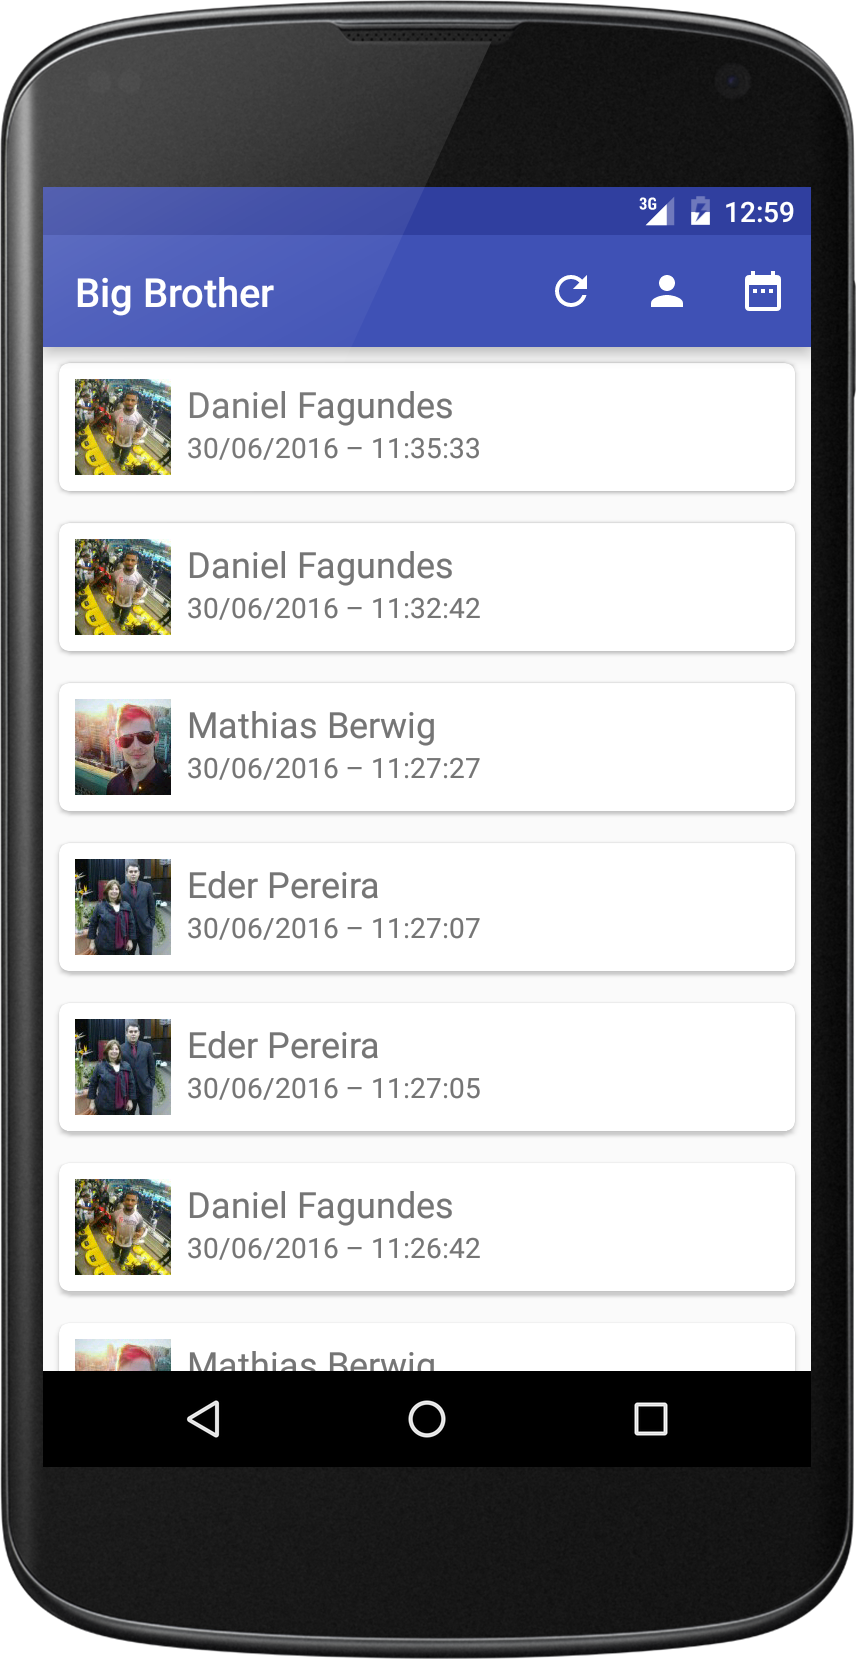
\includegraphics[scale=0.2]{imagens/android_tela_inicial.png}
	\label{android_tela_inicial}
\end{subfigure}%
\begin{subfigure}{.5\textwidth}
	\centering
	\caption{Opção Filtrar Pessoas}
	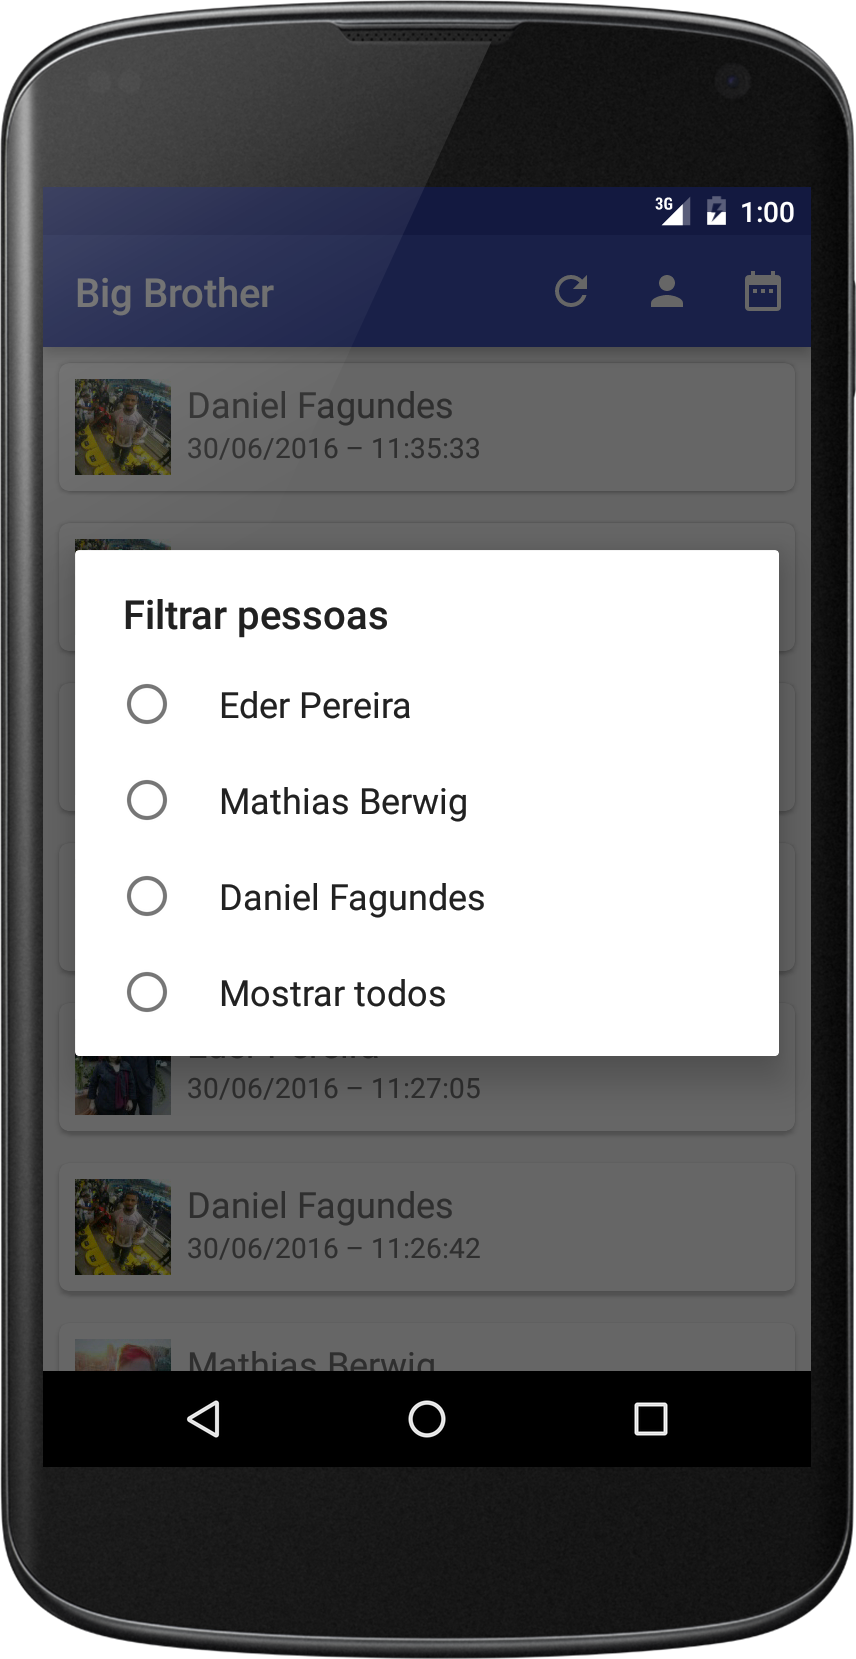
\includegraphics[scale=0.2]{imagens/android_filtrar_pessoas.png}
	\label{android_filtrar_pessoas}
\end{subfigure}
\begin{subfigure}{.5\textwidth}
	\centering
	\caption{Opção Filtrar Datas}
	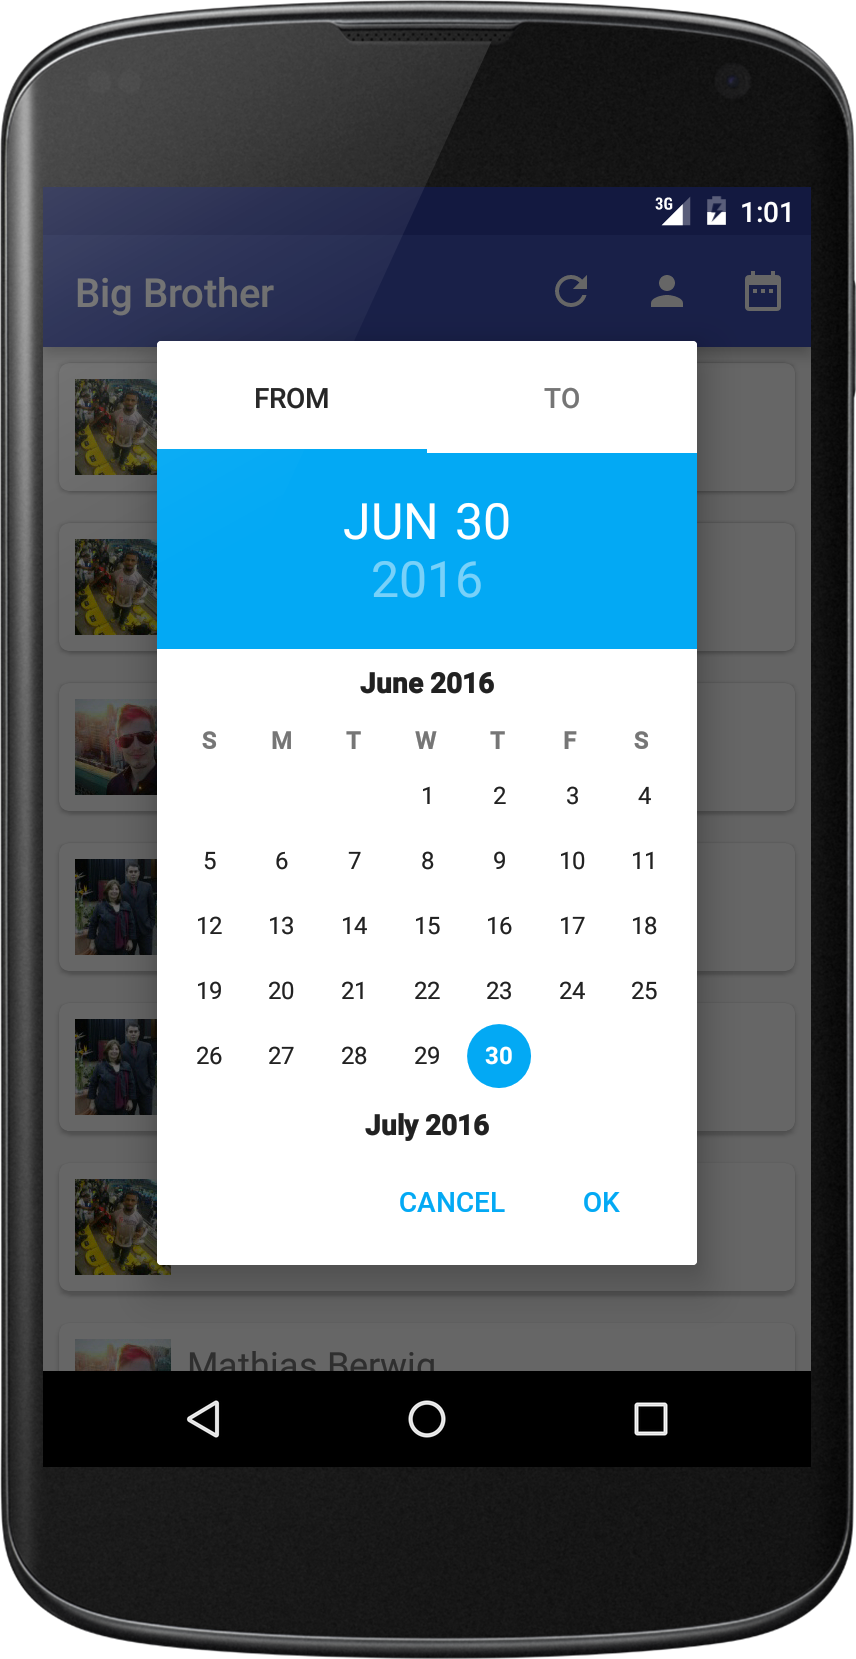
\includegraphics[scale=0.2]{imagens/android_filtrar_data.png}
	\label{android_filtrar_data}
\end{subfigure}
\caption{Capturas de tela do aplicativo.}
\label{android_screenshots}
\end{figure}
\chapter{Conclusão}
\label{conclusao}

A implementação das funcionalidades solicitadas foi cumprida, visto que o sistema é capaz de ler cartões com suporte a RFID, registar as leituras no servidor e exibir ao usuário por meio do aplicativo para Android. O projeto se mostrou uma alternativa simples e barata para o controle de ponto na universidade.

O desenvolvimento apresentado primou pela simplicidade, o que nem sempre é a melhor alternativa para sistemas de utilizados em ambiente de produção. Para tal, seriam necessários diversos ajustes de modo a tornar o sistema mais seguro e resistente à falhas, além de adapta-lo ao sistema utilizado na universidade.

Atividades práticas são muito importantes para o desenvolvimento das habilidades de estudantes, podendo ser o diferencial na experiência profissional dos mesmos. Deste modo, o autor considera que construir protótipos como este é uma tarefa claramente benéfica ao aprendizado dos alunos.

\postextual

% ----------------------------------------------------------
%Referências bibliográficas
% ----------------------------------------------------------
% \bibliography{referencias.bib}


\end{document}
